%!TEX root = thesis.tex
%% %% ***************** Machine learning pipeline structure *****************

%% ************************************************ 4 ************************************************

\section{Machine learning pipeline structure}\label{sec:ml-pipeline}

The full component chain from input to output
with algorithm training and result validating
is called a machine learning pipeline.
In this section,
we discuss how ML pipeline was created in Azure ML Studio.
Several ML algorithms were compared
in order to find the most feasible set for our goal in mind.
ML training was organized in two different phases
in order to find the relation between
log anomalies and technical tickets.
Although the Azure environment and ML Studio requirements
were the objectives of the study and therefore part of the outcome of the results,
these results were also a prerequisite for solving the final objective
considering the ML algorithm possibilities.
Therefore,
the resulting Azure resources and ML Studio pipeline components
are demonstrated in this section.

Results of the trained algorithms
were validated against newly acquired production data
in order to estimate how well the initial goals of the study
were fulfilled.
These results are presented later in section~\ref{sec:results}.

Azure ML Studio makes ML pipeline creation easy
and comparing different methods and algorithms effortless.
Nevertheless,
with hybrid approach having two different phases,
and result comparison being done against anomaly hypothesis,
the pipeline drafts started to accumulate in content.

When starting the ML pipeline testing
the initial plan was to feed the log data to anomaly detection algorithm
and try to get some sort of estimate of possible anomaly count.
This plan had several problems.
First, as stated, logging is very abundant
and several thousands of rows is logged
during a single day.
Some errors encountered are not critical
and RPA agent is able to recover from them
finalizing the initial task.
This means,
that errors which could be deemed anomalous
may not result to a ticket in the end.

In addition,
one single error case noticed by bank clerks
may be linked to several problems in runtime,
meaning that one ticket received is,
in fact, linked to multiple, dozens, or
even hundreds of log rows.

Two different algorithms were needed.
In phase 1,
algorithm defines how likely one datapoint, or log row,
is to be considered an anomaly.
In phase 2,
another algorithm aims to predict
how many tickets are to be expected to receive
within a time frame.
This dual algorithm utilization is referred as a hybrid machine learning approach.~\cite{tsai2010credit}



%% TODO: find place and something to say
\begin{figure}[htb]
    \centering
    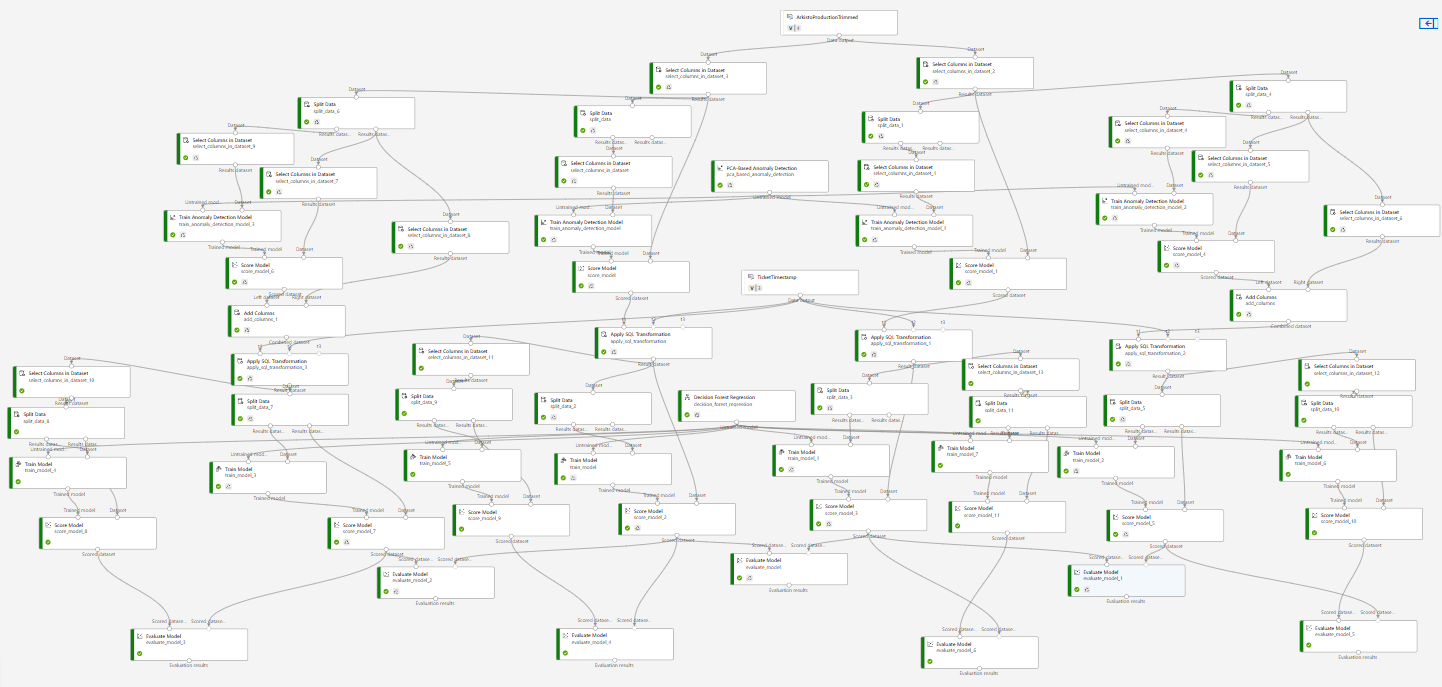
\includegraphics[width=150mm]{./appendices/pipeline-draft}
    \caption{TODO: Pipeline in all its glory. Find a better place and edit caption.
    \label{fig:pipeline draft}}
\end{figure}

%% ************************************************************************************************************


\subsection{Feature format for PCA-ADA}\label{subsec:pipe-pca-ada-feature-format}

In Azure ML Studio
there is only one module selectable
for anomaly detecting,
the PCA-based anomaly detection module,
which is explained in section~\ref{subsec:bg-pca-ada}.
However,
with textual input like logs
it can be used at least in two ways.
First,
input data can be fed to
the algorithm trainer as is,
letting the PCA-based anomaly detection algorithm (ADA) component
do the work without further modifying the log rows.
This way,
the component tries to recognize the anomalies
based on all the information included in the row.
Practically this means,
that the component processes data in textual format
making each row in the input
a feature as a whole
to consider.

Second option is to convert the textual features into numerical features.
This can be done
either with "Extract N-Gram Features from Text" component,
or "Feature Hashing" component.
With n-gram feature extracting,
each word or n-gram
is converted to a number of said instance found on the row being processed,
and each row can be presented as a sequence of numbers
indicating the number of those features.

N-gram feature can in addition have a weight
based on the frequency n-grams appear
in the entire data.
Different weights usable in Azure ML component
are listed in the table~\ref{tab:n-gram-weights}.
During this study,
only binary weight was used,
so it is possible that improved results could have acquired with different weight method.

\begin{table}[]
    \begin{tabularx}{\textwidth}{|L{0.25\textwidth}|Y|}
        \hline
        \textbf{N-gram weight}  & \textbf{Explanation}       \\ \hline
        Binary Weight       & Assigns a binary presence value to the extracted n-grams. The value for each n-gram is 1 when it exists in the document, and 0 otherwise.     \\ \hline
        TF Weight           & Assigns a term frequency (TF) score to the extracted n-grams. The value for each n-gram is its occurrence frequency in the document.                \\ \hline
        IDF Weight          & Assigns an inverse document frequency (IDF) score to the extracted n-grams. The value for each n-gram is the log of corpus size divided by its occurrence frequency in the whole corpus. \verb-IDF = log of corpus_size / document_frequency-        \\ \hline
        TF-IDF Weight       & Assigns a term frequency/inverse document frequency (TF/IDF) score to the extracted n-grams. The value for each n-gram is its TF score multiplied by its IDF score.      \\ \hline
    \end{tabularx}
    \caption{Statistic metrics of the time frame compression that are considered possibly useful for ML algorithm.~\cite{azure2021ngramfeature}}
    \label{tab:n-gram-weights}
\end{table}



%% TODO: this should be explained in the background!
Vast dictionary of n-grams demands resources from the ML computing instances
as every new n-gram in the dictionary adds another column to the training dataset.
To reduce the amount of memory needed,
Azure ML Studio has "Feature Hashing" component.

By hashing the n-gram features,
the amount of resources needed by the pipeline
can be significantly reduced.
Feature hashing allows us to use the whole amount of data as an input
if feature hashing parameters are tuned enough.
As explained previously in the section~\ref{subsec:bg-ngram-features-and-hashing},
the greater the compression is,
the more information is lost
while resources needed are reduced.

%% TODO: Results/parameters used in n-gram and feature hashing!




%% TODO: RESULTS:
%   Pure n-gram feature component using skipped
%   Only 2% of the data could be used. Not enough.
%


%% ************************************************************************************************************

%% TODO:!!!
\subsection{Anomaly probability}\label{subsec:pipe-anomaly-probability}
%% TODO: PCA output
\begin{itcomment}
    Here we explain what PCA-component outputs and how the result is used in the pipeline.
\end{itcomment}

The output values of the PCA-ADA component are
%, as explained in the section~\ref{subsec:bg-pca-ada}, %% TODO:?!?
normalized so the values range between 0 and 1.
This anomaly probability value
is the main output of hybrid ML phase 1.
Based on our initial hypothesis
that each anomalous event in the log
is linked to a real life support ticket received,
the bigger a single anomaly probability value is for a log row
the more likely that row is related to a ticket inducing event.


%% ************************************************************************************************************


\subsection{Unconventional training approach}\label{subsec:pipe-unconventional-training}

As stated in section~\ref{subsec:bg-machine-learning},
the approach used in this study is,
if expression is allowed, unorthodox.
Typically,
data points used in ML algorithm training and validating
should always be different.
Acting otherwise leads to algorithm processing with
same data it was trained with,
thus creating a situation
where algorithm already knows what to do with the current data point.
If the results were validated after this
the algorithm would get unreliable score
as it had the validation data already in the training phase.
This could be compared to
giving some right answers to students during test
and scoring test results as if no help was given.
However,
due to the nature of the study problem and contents of the data,
it was decided to test whether bending this rule
would provide better results in algorithm training.

Even though the amount of data was large enough
to cause issues with memory,
the hybrid approach and the time frame compression discussed <later in this section> %% TODO: check!
lead to significant reduction of data in phase 2.
As a general rule of thumb in ML training,
only 20--30\% of the data is used to validate the algorithm.
With the hybrid ML approach,
the validation results in phase 1
are what actually form the data used in the phase 2.
This data is further compressed to time frame groups
leading to only a few dozen data points in phase 2 ML training %% TODO: more accurate numbers?
compared to millions of rows in phase 1.

Because of the way the anomaly detection algorithms work
the over-lapping data points are not as big of an issue
as it would be with other types of algorithms
like regression algorithms. %% TODO: do they though?
This is why we could use part of the data
for training the anomaly detection algorithm as usual
and then use all the data available for validation
without overfitting the algorithm. %% TODO: check and refer to something?
Also, because the main forecasting functionality comes in the phase 2,
overtraining %% TODO: check wording
in phase 1 may not cause issues. %% TODO: phrasing?

To verify if this unconventional training method gives good results without issues,
the trained algorithms were tested with new production data
that had zero overlapping data points with training and validation data.
This way we were able to compare different training approaches
to determine the best overall pipeline.


%% ************************************************************************************************************



%% TODO: Mention that data splits in phase 1 have to be un-random
%% Otherwise, possible anomaly values used in phase 2 would be randomly included
%% Data in phase 1 need to be chronological!


%% TODO: Results: Feature Hashing runs out of memory in Model Training with full data (unconventional training)
%% Trying with smaller splits, which, once again, reduces data amount.



%% ************************************************************************************************************

\subsection{Input data random delay and time frame compression}\label{subsec:pipe-random-delay-and-timeframe-compression}

As mentioned previously in the section~\ref{sec:introduction},
it takes time for bank clerk to notice the error in RPA process,
send a technical support ticket considering the issue,
and support team to redirect the request to corresponding developer team.
As several steps of human interaction and workday schedules
are in between the event logging and ticket receiving,
the random delay of such may span from hours to days.
Random delay in input data features
is not unusual aspect in time-series forecasting.
Time-series in ML context
refers to data features that varies over time
and can be affected by past values.~\cite{palma2016time}
As an example,
ML algorithm could try to predict future weather
based on measured temperature and air pressure.
Both these features change over time
and also affect to their own future values.

This study, however,
is not about time-series
because the majority of the log rows
are not affected by previously logged events.
As random delay of such
does not seem to be trivial to take into account
with ML algorithms,
a simple method to solve this was used
where log rows were grouped by time stamp
into certain time frame groups.
We call this method \enquote{time frame compression method}.

Time frame compression means,
that in order to eliminate the effects of random delay
we compress some features in certain time frame
which is at least as long as the longest estimated delay.
Simply put,
if we count possible anomalies during one hour of log,
we cannot compare this number to actual tickets received
at the same hour or the next.
What we can do,
with time frame compression,
is that we count some statistical values of anomaly estimates,
for example, the mean and median values of a week,
and then compare these numbers with the tickets received
during the same week.
Statistically important and thus compressed features of a time frame
were determined to be the log row count,
amount of unique job IDs, and anomaly probability metrics.

The amount of log rows describes
how much logged issues happened in a time frame.
Alone,
this feature may not give much insight
as the amount of logs is possibly not linearly comparable
to the amount of tickets received.
Combined to other statistical metrics
it may, however,
provide additional value for ticket forecasting.
Job ID is the identification information of a specific RPA automation execution run.
It means,
that job ID is not unique for each log row,
but it binds together all the log entries on the same RPA automation execution.
By counting the amount of unique job IDs in a time frame
we can get insight about the amount of jobs executed during the time frame.
This metric is important with the total row count:
low number of unique jobs with high number of total rows
indicates that plenty of loggable events and possibly errors happened during the time frame,
whereas high number of unique jobs combined to low number of rows
imply that not much happened (or perhaps executions were completely crashed).

By the original hypothesis,
anomalies in the logs are linked closely to the support tickets received.
Anomaly detection algorithm produces a probability value of
how strongly a row is suspected to be an anomaly,
thus,
mean and median values of the anomaly probabilities in a time frame
indicate how anomalous all the executions on a time frame has statistically been.
However,
when compressing the anomaly probability metrics in a time frame,
some information is bound to be lost.
Mean and median values do not provide information
about the anomaly probability value distribution.
There may be few very high values and a lot of low probabilities,
and it would lead to the same mean value
as there were a lot of slightly higher probabilities and just few very low values.
By adding more statistical values
we can reduce the loss of information caused by time frame compression.
If the original hypothesis is correct,
the most relevant anomaly values are the highest anomaly probabilities.
Thus,
calculating higher quantiles and the amount of values exceeding them
should improve the estimation abilities of the algorithm.

\begin{table}[]
    \begin{tabularx}{\textwidth}{|L{0.4\textwidth}|Y|}
        \hline
        \textbf{Statistic feature}  & \textbf{Explanation (in time frame)}       \\ \hline
        LogRowCount              & Number of rows/instances overall           \\ \hline
        UniqueJobIDs             & Amount of unique job IDs                   \\ \hline
        AnomalyProbabilityMean   & Mean value of anomaly probabilities        \\ \hline
        AnomalyProbabilityMedian & Median value of anomaly probabilities      \\ \hline
        AnomalyQuantile90        & 90-quantile value of anomaly probabilities \\ \hline
        AnomalyCountOverQ90 & Number of instances with anomaly probability over 90-quantile \\ \hline
    \end{tabularx}
    \caption{Statistic metrics of the time frame compression that are considered possibly useful for ML algorithm.}
    \label{tab:statistic-features}
\end{table}

In the table~\ref{tab:statistic-features},
all the statistic metrics considered interesting and valuable
from time frame compression of the log rows
are listed with short explanation.
In the pipeline,
the statistical values are calculated
using component executing R-script.
An example of such script executed by the "Execute R Script" component
is presented in the appendix~\ref{sec:app-r-script}.


%% ************************************************************************************************************


\subsection{Regression based estimating}\label{subsec:pipe-regression-estimating}
%% TODO: parameters?
%% Ticket amount forecasting
\begin{itcomment}
    Here is more information about different regression algorithms
    used in ML pipeline.
    Some basic information about all of them is given so the results are understandable
    by reader in the Result section.
\end{itcomment}

\begin{enumerate}
    \item Linear regression
    \item Decision forest regression
    \item Neural network regression
    \item Boosted decision tree regression
\end{enumerate}


%% ************************************************************************************************************


\subsection{Pipeline branching}\label{subsec:pipe-branching}

%In the methods section
%we discussed of different approaches that could be used
%to get the best results from the ML training.
In order to compare different results,
some comparable metrics are needed.
%% TODO: declare comparable metrics etc.

Several diverging points caused the pipeline to branch.
First,
the error message used to calculate the anomaly probability of a log row
had two options.
We could either use simple \textit{message},
or more verbose \textit{rawmessage}.
This textual data could be fed to the ADA-component in several forms.
Most straightforward way was using textual data without any preformatting.
Text could also be run through \enquote{Preprocess text} -component. %% TODO: Explain somewhere!
N-gram features could have been extracted from the text
and these features could have been used instead.
Instead of n-gram features,
textual data could be converted to numeric
with \enquote{Feature Hashing} -component.
After getting the ADA-component results,
the anomaly probabilities were compressed with R-code or SQL. %% TODO: ?
<This concludes the phase 1.> %% TODO: ??

In phase two,
branching of the pipeline was due to either different regression algorithms used
or comparing results without the anomaly probability values calculated in phase 1.
In practice this means
that in order to validate the results against our initial hypothesis,
we used pure statistical log data such as row count and unique job ID count
without anomaly probabilities
to determine whether anomaly metrics provided any insight regarding the ticket data.

Each branching step, or layer,
multiplies the amount of results used in final comparison
that would determine the best possible pipeline combination.
These layers are simplified in the table~\ref{tab:ml-pipeline-branching}.

\begin{table}[]
    \centering
    \begin{tabularx}{\textwidth}{|L{0.3\textwidth}|L{0.45\textwidth}|X|}
        \hline
        \textbf{Branching node}           & \textbf{Options}                                                              & \textbf{Layer count} \\ \hline
        Input text column                  & \begin{tabular}[c]{@{}l@{}}message \\ rawmessage\end{tabular}                 & 2                        \\ \hline
        Text preprocess                    & \begin{tabular}[c]{@{}l@{}}Yes\\ No\end{tabular}                              & 2                        \\ \hline
        Numeric conversion                 & \begin{tabular}[c]{@{}l@{}}No\\ N-gram Feature\\ Feature Hashing\end{tabular} & 3                        \\ \hline
        ADA training                       & \begin{tabular}[c]{@{}l@{}}Unconventional \\ Proper\end{tabular}              & 2                        \\ \hline
        Validation without anomaly metrics & \begin{tabular}[c]{@{}l@{}}Yes\\ No\end{tabular}                           & 2                        \\ \hline
        Regression algorithms &
        \begin{tabular}[c]{@{}l@{}}Decision forest regression \\ Boosted decision tree regression \\ Neural Network Regression \\ Linear regression\end{tabular} &
        4 \\ \hline
    \end{tabularx}
    \caption{Pipeline divergent layers}
    \label{tab:ml-pipeline-branching}
\end{table}

The divergent count implies the number of branches
diverging from the previous component.
The total count of branch ends, or leaves,
would then be the multiplication of all divergent counts,
totaling to 192 comparable pipeline combinations.
Moreover,
n-gram feature extraction and feature hashing
have several tunable parameters
that strongly influence the end results of the algorithm training.
To reduce this amount when considering the best possible pipeline,
we simplified this by narrowing down the options
based on initial test run results of some of the divergent options.

For example,
n-gram feature component suffered greatly from the memory problem %% TODO: refer to it?
and the data amount that the \textit{Extract N-Gram Features from Text} -component
was able to handle only 2\% of the original data amount.
This was deemed as too small amount for training
as it would be extremely likely with 98\% of the data skipped
that also possible rows relevant to the ticket anomalies
would get trimmed out.



%% TODO: unorganized text below!

%% TODO: Next up is outdated
%
%Usually <with usual ml methods> the estimates
%created using ML algorithms
%are formed based on the certain features
%presented on a one element of the data,
%or on one row.
%This means that in typical case,
%there is one column in the data
%given to the ML algorithm
%that is removed from the training data
%and this column value is what algorithm
%aims to predict.
%
%In this study case, however,
%data does not contain clear values
%that are being estimated
%and that can be used as comparison.
%
%\begin{tabular}{cccc}
%    LOG\_DATA \\
%    a=date & b=msg & c=\etc & \\
%    a & b & c & n1 \\
%    a & b & c & n2 \\
%    a & b & c & n3 \\
%    a & b & c & n4
%\end{tabular}
%
%\begin{tabular}{c}
%    EFECTE\_DATA \\
%    A YYYY.MM.DD hh:mm:ss \\
%    B YYYY.MM.DD hh:mm:ss \\
%    C YYYY.MM.DD hh:mm:ss \\
%    D YYYY.MM.DD hh:mm:ss \\
%    E YYYY.MM.DD hh:mm:ss
%\end{tabular}
%\\
%n1 = SUM(AB) \\
%n2 = SUM(C) \\
%n3 = SUM(DE) \\
%=> \\
%We could try to predict nx
%but usually this is done
%by making estimate based on
%a, b and c.
%Instead,
%we aim to estimate the sum of events
%in timeframe.
%We should also skip event instances
%that are close to each other
%to avoid counting multiple values
%linked to same error
%as different possible ticket creators.




\clearpage